\documentclass[english,brazil]{article}

\usepackage{mathptmx}
\renewcommand{\ttdefault}{mathptmx}
\usepackage[utf8]{inputenc} %Usar UTF8
\usepackage[a4paper]{geometry} %Imprimir em a4
\geometry{verbose,tmargin=2.5cm,bmargin=2.5cm,lmargin=3cm,rmargin=3cm} %Aumenta um pouco a margem, principalmente a inferior
\setlength{\parindent}{10mm}
\usepackage{float}
\usepackage{units}
%Bibliotecas para fazer formulas e transforma-las em "objetos"
\usepackage{amsmath}
\usepackage{amssymb}
\usepackage{graphicx} % Poder inserir imagens
\makeatletter
\usepackage{changepage} %Para poder usar adjustwidth
\providecommand{\tabularnewline}{\\}
\newcommand{\lyxdot}{.}
\usepackage[brazilian]{babel} %Imprimir em português Ex. Tabela x
\usepackage[11pt]{moresize}% different letters sizes
\usepackage{caption}% to make personalized captions

\title{Experimento 5  \\ Viscosidade: Lei de Stokes } % main title
\author{F 229 \\ \textsc{Grupo 1}}
\date{19 de Novembro, 2014}

\makeatother

\usepackage{babel}
\begin{document}

	 \maketitle

	% members of the group


	\begin{center}
		\begin{tabular}{rr}
			                    Integrantes:  & \tabularnewline
			                                  & \tabularnewline
			        Henrique Noronha Facioli  & RA: 157986 \tabularnewline
			        Guilherme Lucas da Silva  & RA: 155618 \tabularnewline
			          Beatriz Sechin Zazulla  & RA: 154779 \tabularnewline
			              Lucas Alves Racoci  & RA: 156331 \tabularnewline
			Isadora Sophia Garcia Rodopoulos  & RA :158018 \tabularnewline
		\end{tabular}
	\par\end{center}

	%%Seria legal se alguém conseguir colocar os logos no footer da pagina, ou então no header...


	\begin{figure}[!ht]
		\begin{minipage}[b]{0.45\linewidth}
			
\includegraphics[scale=0.25]{logo-unicamp-name-line-blk-blk-0480.jpg}
		\end{minipage}
		\hspace{0.5cm}
		\begin{minipage}[b]{0.45\linewidth}
			
\includegraphics[scale=0.25]{logo-ifgw.png}
		\end{minipage}
	\end{figure}



	\newpage{}


\section{Resumo}

	A partir do fenômeno de movimento de um corpo em meio viscoso, o experimento visa investigá-lo pelo comportamento da velocidade de diversas esferas em um tubo de vidro com glicerina e água. Uma esfera em um meio viscoso possui três forças atuando sobre ela: força do peso, força do empuxo e a força da viscosidade. 

Sabendo a fórmula da força de empuxo $F_E = \cfrac{g \rho ' 4 \pi r^3}{3}$, com $g$ sendo a aceleração da gravidade (dada por 9,8 +/- 0,2 m/s$^2$), $\rho '$ a densidade do meio e $r$ o raio da esfera; a força peso $F_P =  \cfrac{g \rho 4 \pi r^3}{3}$, com $\rho$ sendo a densidade da esfera; e a força de viscosidade $F_V = 6\pi \eta r v$, com $\eta$ sendo o coeficiente de viscosidade do meio e $v$ a velocidade da esfera - é possivel concluir que, quando a resultante dessas forças for igual a zero, o corpo terá atingido a velocidade limite. Sendo, então, apresentada por:

\begin{equation}
	v_L = \cfrac{2}{9} \cdot \bigg[\cfrac{\rho - \rho '}{\eta}\bigg] \cdot g r^2
\end{equation}

Entretanto, como estamos lidando com um meio viscoso em um tubo, a força viscosa deve ser corrigida com o fator de Ladenburg $K = \bigg(\cfrac{1 + 2,4r}{A}\bigg) \cdot \bigg(\cfrac{1 + 3,3r}{H}\bigg)$, em que $A$ é o raio do tubo e $H$ é a altura total do fluido no tubo. Para corrigí-la, basta multiplicá-la por $K$, resultando na velocidade mais precisa $v_L$ a partir da velocidade medida $v'_L$

\begin{equation}
	v_L = K v_L ' = \cfrac{2}{9} \cdot \bigg[\cfrac{\rho - \rho '}{\eta}\bigg] \cdot g r^2
\end{equation}

Dispostos dessas equações, simulou-se a queda de diversas esferas no tubo de vidro - qualificando os valores de altura, tempo e propriedades da esfera. Com a manipulação desses dados, foi possível encontrar o coeficiente de viscosidade do meio $\eta$ com o valor de $8 \cdot 10^{-1}$ +/- $2 \cdot 10^{-1}$ Pa$\cdot$s, qualificando as propriedades da viscosidade da mistura de glicerina e água e que, por sua vez, permitiu concluir uma concentracão de água na mistura de $(95\pm5)\%$.

\section{Objetivo}

	O experimento visa investigar o movimento de corpos em meios viscosos, determinar o percentual de água na glicerina e a viscosidade da mistura. Tais objetivos serão atingidos através da manipulação dos dados experimentais, e da consequente linerarizacão da função em contraste com a equação (2).


\section{Procedimentos e coleta de dados}


	\subsection{Materiais utilizados}
		\begin{enumerate}
			\item Tubo de vidro com uma mistura de agua e glicerina 
			\item Suporte com marcas graduadas 
			\item Conjunto de esferas 
			\item Paquímetro 
			\item Micrômetro 
			\item Cronômetro 
			\item Termômetro de mercúrio 
		\end{enumerate}

	\begin{figure}[!ht]
		\centering
		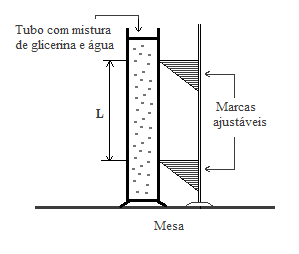
\includegraphics[scale=0.8]{arranjo-experimental.png}
		\caption{Montagem do experimento}
	\end{figure}

	\subsection{Procedimento}

		Para realização do experimento, um tubo de vidro foi preenchido com uma mistura de água de glicerina e foi colocado duas hastes, separadas por uma régua graduada, de modo que pudéssemos saber a distância da haste superior até a haste inferior e que, quando as esferas atingissem a haste superior, elas já estariam com sua velocidade limite. Pegamos 5 esferas metálicas maciças $a,b,c,d,e$ de diâmetros diferentes (cujos diâmetros estão expressos na Tabela 2) e a colocávamos dentro do líquido e cronometramos o tempo que elas demoravam para atingir a haste inferior (cujos os dados estão na Tabela 3).
		
		\begin{table}[!ht]
			\caption{Dados sobre o tubo de água com glicerina}
			\centering{}%
				\begin{tabular}{|r|rl|}
					\hline 
					Diametro do Tubo  & $(5,325\pm0,005)$  & \selectlanguage{english}%
					$\cdot10^{-2}\unit{m}$\selectlanguage{brazil}%
					\tabularnewline
					\hline 
					Diferença de altura das hastes  & $(3,000\pm0,005)$  & $\cdot10^{-1}\unit{m}$\tabularnewline
					\hline 
					Temperatura da mistura & $(2,60\pm0,05)$  & $\cdot10^{1}\unit{^{\circ}C}$\tabularnewline
					\hline 
				\end{tabular}
		\end{table}
		
		\begin{table}[!ht]
			\caption{Diâmetros das esferas}
			\centering{}%
			\begin{tabular}{|c|c|}
				\hline 
				Esfera  & Diametro das Esferas \tabularnewline
				\hline 
				a  & $(2,0\pm0,5)\cdot10^{-3}\unit{m}$\tabularnewline
				\hline 
				b  & $(2,5\pm0,5)\cdot10^{-3}\unit{m}$\tabularnewline
				\hline 
				c  & $(3,0\pm0,5)\cdot10^{-3}\unit{m}$\tabularnewline
				\hline 
				d  & $(3,5\pm0,5)\cdot10^{-3}\unit{m}$\tabularnewline
				\hline 
				e  & $(4,0\pm0,5)\cdot10^{-3}\unit{m}$\tabularnewline
				\hline 
			\end{tabular}
		\end{table}

		\begin{table}[!ht]
			\begin{adjustwidth}{-1.5cm}{-1cm}
			\caption{Tempos de queda de cada esfera pra cada uma das $N=5$ medidas realizadas (i.e. $t_{ki}$ é o tempo de queda da k-ésima esfera na i-ésima medição)}
			\centering{}%
			\begin{tabular}{|c|cc|cc|cc|cc|cc|}
				\hline 
				$i$  & $t_{ai}$  &  & $t_{bi}$  &  & \selectlanguage{english}%
				$t_{ci}$\selectlanguage{brazil}%
				 &  & \selectlanguage{english}%
				$t_{di}$\selectlanguage{brazil}%
				 &  & \selectlanguage{english}%
				$t_{ei}$\selectlanguage{brazil}%
				 & \tabularnewline
				\hline 
				$1$  & $(1,713\pm0,001)$  & \selectlanguage{english}%
				$\cdot10^{1}\unit{s}$\selectlanguage{brazil}%
				 & $(1,146\pm0,001)$  & \selectlanguage{english}%
				$\cdot10^{1}\unit{s}$\selectlanguage{brazil}%
				 & $(8,19\pm0,01)$  & \selectlanguage{english}%
				$\cdot\unit{s}$\selectlanguage{brazil}%
				 & $(6,06\pm0,01)$  & \selectlanguage{english}%
				$\cdot\unit{s}$\selectlanguage{brazil}%
				 & $(4,87\pm0,01)$  & \selectlanguage{english}%
				$\cdot\unit{s}$\selectlanguage{brazil}%
				\tabularnewline
				\hline 
				$2$  & $(1,718\pm0,001)$  & \selectlanguage{english}%
				$\cdot10^{1}\unit{s}$\selectlanguage{brazil}%
				 & $(1,150\pm0,001)$  & \selectlanguage{english}%
				$\cdot10^{1}\unit{s}$\selectlanguage{brazil}%
				 & $(8,19\pm0,01)$  & \selectlanguage{english}%
				$\cdot\unit{s}$\selectlanguage{brazil}%
				 & $(6,28\pm0,01)$  & \selectlanguage{english}%
				$\cdot\unit{s}$\selectlanguage{brazil}%
				 & $(4,78\pm0,01)$  & \selectlanguage{english}%
				$\cdot\unit{s}$\selectlanguage{brazil}%
				\tabularnewline
				\hline 
				$3$  & $(1,753\pm0,001)$  & \selectlanguage{english}%
				$\cdot10^{1}\unit{s}$\selectlanguage{brazil}%
				 & $(1,150\pm0,001)$  & \selectlanguage{english}%
				$\cdot10^{1}\unit{s}$\selectlanguage{brazil}%
				 & $(8,21\pm0,01)$  & \selectlanguage{english}%
				$\cdot\unit{s}$\selectlanguage{brazil}%
				 & $(6,06\pm0,01)$  & \selectlanguage{english}%
				$\cdot\unit{s}$\selectlanguage{brazil}%
				 & $(4,75\pm0,01)$  & \selectlanguage{english}%
				$\cdot\unit{s}$\selectlanguage{brazil}%
				\tabularnewline
				\hline 
				$4$  & $(1,734\pm0,001)$  & \selectlanguage{english}%
				$\cdot10^{1}\unit{s}$\selectlanguage{brazil}%
				 & $(1,147\pm0,001)$  & \selectlanguage{english}%
				$\cdot10^{1}\unit{s}$\selectlanguage{brazil}%
				 & $(8,22\pm0,01)$  & \selectlanguage{english}%
				$\cdot\unit{s}$\selectlanguage{brazil}%
				 & $(6,12\pm0,01)$  & \selectlanguage{english}%
				$\cdot\unit{s}$\selectlanguage{brazil}%
				 & $(4,85\pm0,01)$  & \selectlanguage{english}%
				$\cdot\unit{s}$\selectlanguage{brazil}%
				\tabularnewline
				\hline 
				$5$  & $(1,722\pm0,001)$  & \selectlanguage{english}%
				$\cdot10^{1}\unit{s}$\selectlanguage{brazil}%
				 & $(1,138\pm0,001)$  & \selectlanguage{english}%
				$\cdot10^{1}\unit{s}$\selectlanguage{brazil}%
				 & $(8,17\pm0,01)$  & \selectlanguage{english}%
				$\cdot\unit{s}$\selectlanguage{brazil}%
				 & $(6,25\pm0,01)$  & \selectlanguage{english}%
				$\cdot\unit{s}$\selectlanguage{brazil}%
				 & $(4,72\pm0,01)$  & \selectlanguage{english}%
				$\cdot\unit{s}$\selectlanguage{brazil}%
				\tabularnewline
				\hline 
			\end{tabular}
			\end{adjustwidth}
		\end{table}

\section{Análise dos resultados}

	\subsection{Obtendo o tempo médio de queda para cada esfera}

		Para cada esfera k, $k=a,\ldots,e$ tem-se que:
		\begin{equation}
		t_{k}\pm\sigma_{t_{k}}={\displaystyle \underset{t_{k}}{\underbrace{\left(\sum_{i=1}^{N}t_{ki}\right)}}\pm\underset{\sigma_{t_{k}}}{\underbrace{\sqrt{\underset{\sigma_{t_{k_{instrumental}}}^{2}}{\underbrace{0,01^{2}}}+\underset{\sigma_{t_{k_{estat\acute{\imath}stico}}}^{2}}{\underbrace{\cfrac{1}{N}\cdot\cfrac{1}{N-1}\cdot\sum_{i=1}^{N}\left(t_{k}-t_{ki}\right)^{2}}}}}}}
		\end{equation}

		Assim, aplicando essas fórmulas obtém-se:

		\begin{table}[!ht]
			\caption{Tempo de queda médio de cada esfera}
			\centering{}%
			\begin{tabular}{|c|rl|}
				\hline 
				Tempo de queda médio  & Valor  & \tabularnewline
				\hline 
				$t_{a}$  & $(1,728\pm0,007)$  & \selectlanguage{english}%
				$\cdot10^{1}\unit{s}$\selectlanguage{brazil}%
				\tabularnewline
				\hline 
				$t_{b}$  & $(1,146\pm0,002)$  & \selectlanguage{english}%
				$\cdot10^{1}\unit{s}$\selectlanguage{brazil}%
				\tabularnewline
				\hline 
				$t_{c}$  & $(8,20\pm0,01)$  & \selectlanguage{english}%
				$\cdot\unit{s}$\selectlanguage{brazil}%
				\tabularnewline
				\hline 
				$t_{d}$  & $(6,15\pm0,05)$  & \selectlanguage{english}%
				$\cdot\unit{s}$\selectlanguage{brazil}%
				\tabularnewline
				\hline 
				$t_{e}$  & $(4,79\pm0,03)$  & \selectlanguage{english}%
				$\cdot\unit{s}$\selectlanguage{brazil}%
				\tabularnewline
				\hline 
			\end{tabular}
		\end{table}



		\subsection{Cálculo da velocidade $v'_{L}$ através de $t_{k}$e $H$}

			Sabemos que:

			\begin{equation}
				v'_{L}=\cfrac{H}{t_{k}}
			\end{equation}

			e portanto

			$$\sigma_{v'_{L}}=\sqrt{\left(\sigma_{H}\cdot\cfrac{\partial v'_{L}}{\partial H}\right)^{2}+\left(\sigma_{t_{k}}\cdot\cfrac{\partial v'_{L}}{\partial t_{k}}\right)^{2}} = \sqrt{\left(\cfrac{\sigma_{H}}{t_{k}}\right)^{2}+\left(-H\cdot\cfrac{\sigma_{t_{k}}}{t_{k}^{2}}\right)^{2}} $$
			
			
			\begin{equation}
				\sigma_{v'_{L}}=\cfrac{\sqrt{\sigma_{H}^{2}\cdot t_{k}^{2}+H^{2}\cdot\sigma_{t_{k}}^{2}}}{t_{k}^{2}}\label{eq:erro em v'}
			\end{equation}
			
			assim, usando a fórmula obtemos:

			\begin{table}[H]
				\caption{Velocidade $v'_{L}$calculada atravez das fórmulas acima para cada esfera}
				\centering{}%
				\begin{tabular}{|c|rl|}
					\hline 
					Esfera  & $v'_{L}$  & \tabularnewline
					\hline 
					a  & $(1,736\pm0,008)$  & \selectlanguage{english}%
					$\cdot10^{-2}\unitfrac{m}{s}$\selectlanguage{brazil}%
					\tabularnewline
					\hline 
					b  & $(2,617\pm0,007)$  & \selectlanguage{english}%
					$\cdot10^{-2}\unitfrac{m}{s}$\selectlanguage{brazil}%
					\tabularnewline
					\hline 
					c  & $(3,658\pm0,009)$  & \selectlanguage{english}%
					$\cdot10^{-2}\unitfrac{m}{s}$\selectlanguage{brazil}%
					\tabularnewline
					\hline 
					d  & $(4,88\pm0,04)$  & \selectlanguage{english}%
					$\cdot10^{-2}\unitfrac{m}{s}$\selectlanguage{brazil}%
					\tabularnewline
					\hline 
					e  & $(6,26\pm0,04)$  & \selectlanguage{english}%
					$\cdot10^{-2}\unitfrac{m}{s}$\selectlanguage{brazil}%
					\tabularnewline
					\hline 
				\end{tabular}
			\end{table}


		\subsection{Cálculo do Fator de Correção de Ladenburg para Cada Esfera}

			O fator de Ladenburg é dado pela fórmula:

			\begin{equation}
				K=\left(1+2,4\cdot\cfrac{r}{R}\right)\cdot\left(1+3,3\cdot\cfrac{r}{h}\right)
			\end{equation}

			cujo erro associado é dado por:

			$$\sigma_{K}=\sqrt{\left(\sigma_{r}\cdot\cfrac{\partial K}{\partial r}\right)^{2}+\left(\sigma_{R}\cdot\cfrac{\partial K}{\partial R}\right)^{2}+\left(\sigma_{h}\cdot\cfrac{\partial K}{\partial h}\right)^{2}}$$

			\begin{equation}
				\hspace{-2cm}\sigma_{K}=\sqrt{\sigma_{h}^{2}\cdot10,89\cdot\cfrac{r^{2}}{h^{4}}\cdot\left(1+2,4\cdot\cfrac{r}{R}\right)^{2}+\sigma_{r}^{2}\cdot\left(\cfrac{1}{h}\left(3.3+7,92\cdot\cfrac{r}{R}\right)+\cfrac{1}{R}\left(2.4+7,92\cdot\cfrac{r}{h}\right)\right)^{2}+\sigma_{R}^{2}\cdot5,76\cdot\cfrac{r^{2}}{R^{4}}\cdot\left(1+3,3\cdot\cfrac{r}{h}\right)^{2}}
			\end{equation}
			

			Portanto aplicando essa fórmula pra cada esfera tem-se que:

			\begin{table}[H]
				\caption{Valores do Fator de Correção de Ladenburg, $K$, calculados à partir dos raios das esferas, do raio do tubo e da altura de liquido}
				\centering{}%
				\begin{tabular}{|c|c|c|}
					\hline 
					Esfera  & Raio das esferas ($r$)  & Fator de Correção de Ladenburg ($K$)\tabularnewline
					\hline 
					a  & $(1,0\pm0,3)\cdot10^{-3}\unit{m}$  & $1,1\pm0,2$\tabularnewline
					\hline 
					b  & $(1,3\pm0,3)\cdot10^{-3}\unit{m}$  & $1,1\pm0,2$\tabularnewline
					\hline 
					c  & $(1,5\pm0,3)\cdot10^{-3}\unit{m}$  & $1,2\pm0,2$\tabularnewline
					\hline 
					d  & $(1,8\pm0,3)\cdot10^{-3}\unit{m}$  & $1,2\pm0,2$\tabularnewline
					\hline 
					e  & $(2,0\pm0,3)\cdot10^{-3}\unit{m}$  & $1,2\pm0,2$\tabularnewline
					\hline 
				\end{tabular}
			\end{table}

		\subsection{Gráfico de $v_{L}\times r^{2}$}

			Tendo a fórmula:
			\begin{equation}
				\underset{y}{\underbrace{v{}_{L}}}=\underset{a}{\underbrace{\cfrac{2}{9}\cdot\cfrac{\rho_{e}-\rho_{f}}{\eta}\cdot g}}\cdot\underset{x}{\underbrace{r^{2}}}+\underset{b}{\underbrace{0}}
			\end{equation}

			Percebemos que para a obtenção do coeficiente de viscosidade essa fórmula é mais útil, porque não fica em função de $K$ portanto calcularemos somente o gráfico de $v_{L}\times r^{2}$, assim, usando a fórmula de mínimos quadrados para erros variáveis em $y$, primeiro calculamos $w_{i}=\cfrac{1}{\sigma_{y_{i}}}$ depois:

			\[
				\begin{cases}
					a & =\frac{\left({\displaystyle {\scriptscriptstyle {\textstyle \overset{n}{\underset{i=1}{\sum}}}}}\left(w_{i}\right)\cdot{\displaystyle {\scriptscriptstyle {\textstyle \overset{n}{\underset{i=1}{\sum}}}}}\left(x_{i}y_{i}w_{i}\right)-{\displaystyle {\scriptscriptstyle {\textstyle \overset{n}{\underset{i=1}{\sum}}}}}\left(x_{i}w_{i}\right){\scriptscriptstyle {\textstyle \overset{n}{\cdot\underset{i=1}{\sum}}}}\left(y_{i}w_{i}\right)\right)}{{\displaystyle {\scriptscriptstyle {\textstyle \overset{n}{\underset{i=1}{\sum}}}}}\left(w_{i}\right)\cdot{\displaystyle {\scriptscriptstyle {\textstyle \overset{n}{\underset{i=1}{\sum}}}}}\left(x_{i}^{2}w_{i}\right)-\left({\displaystyle {\scriptscriptstyle {\textstyle \overset{n}{\underset{i=1}{\sum}}}}}\left(x_{i}w_{i}\right)\right)^{2}}\pm\sqrt{\cfrac{{\displaystyle {\scriptscriptstyle {\textstyle \overset{n}{\underset{i=1}{\sum}}}}}\left(w_{i}\right)}{{\displaystyle {\scriptscriptstyle {\textstyle \overset{n}{\underset{i=1}{\sum}}}}}\left(w_{i}\right)\cdot{\displaystyle {\scriptscriptstyle {\textstyle \overset{n}{\underset{i=1}{\sum}}}}}\left(x_{i}^{2}w_{i}\right)-\left({\displaystyle {\scriptscriptstyle {\textstyle \overset{n}{\underset{i=1}{\sum}}}}}\left(x_{i}w_{i}\right)\right)^{2}}}\\
					b & =\frac{\left({\displaystyle {\scriptscriptstyle {\textstyle \overset{n}{\underset{i=1}{\sum}}}}}\left(y_{i}w_{i}\right)\cdot{\displaystyle {\scriptscriptstyle {\textstyle \overset{n}{\underset{i=1}{\sum}}}}}\left(x_{i}^{2}w_{i}\right)-{\displaystyle {\scriptscriptstyle {\textstyle \overset{n}{\underset{i=1}{\sum}}}}}\left(x_{i}y_{i}w_{i}\right){\scriptscriptstyle {\textstyle \overset{n}{\cdot\underset{i=1}{\sum}}}}\left(x_{i}w_{i}\right)\right)}{{\displaystyle {\scriptscriptstyle {\textstyle \overset{n}{\underset{i=1}{\sum}}}}}\left(w_{i}\right)\cdot{\displaystyle {\scriptscriptstyle {\textstyle \overset{n}{\underset{i=1}{\sum}}}}}\left(x_{i}^{2}w_{i}\right)-\left({\displaystyle {\scriptscriptstyle {\textstyle \overset{n}{\underset{i=1}{\sum}}}}}\left(x_{i}w_{i}\right)\right)^{2}}\pm\sqrt{\cfrac{{\displaystyle {\scriptscriptstyle {\textstyle \overset{n}{\underset{i=1}{\sum}}}}}\left(x_{i}^{2}w_{i}\right)}{{\displaystyle {\scriptscriptstyle {\textstyle \overset{n}{\underset{i=1}{\sum}}}}}\left(w_{i}\right)\cdot{\displaystyle {\scriptscriptstyle {\textstyle \overset{n}{\underset{i=1}{\sum}}}}}\left(x_{i}^{2}w_{i}\right)-\left({\displaystyle {\scriptscriptstyle {\textstyle \overset{n}{\underset{i=1}{\sum}}}}}\left(x_{i}w_{i}\right)\right)^{2}}}
				\end{cases}
			\]

			Achamos:

			\[
				\begin{cases}
					a & =\left(1,9\pm0,4\right)\cdot10^{4}\cdot\unit{\left[s\cdot m\right]^{-1}}\\
					b & =\left(3,9\pm0,7\right)\cdot10^{-3}\cdot\unit{\unitfrac{m}{s}}
				\end{cases}
			\]
			
			Traçando o gráfico:
			\begin{figure}[!ht]
				\centering
					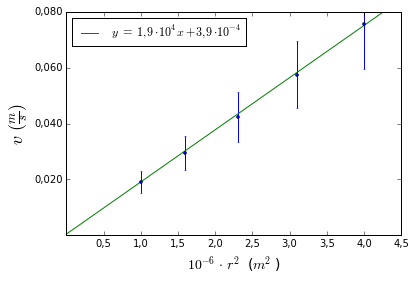
\includegraphics[scale=0.747]{exp05-vcorrigida.png}
				\caption{Gráfico de $v_{L}\times r^{2}$}
			\end{figure}


		\subsection{Obtenção do Coeficiente de Viscosidade ($\eta\pm\sigma_{\eta}$)}

			Sabemos que 
			$$a=\cfrac{2}{9}\cdot\cfrac{\rho_{e}-\rho_{f}}{\eta}\cdot g\Leftrightarrow$$
		
		\begin{equation}
			\eta=\cfrac{2}{9}\cdot\cfrac{\rho_{e}-\rho_{f}}{a}\cdot g=\cfrac{2}{9}\cdot\left(\rho_{e}-\rho_{f}\right)\cdot\cfrac{g}{a}
		\end{equation}

			assim 
			
			$$\sigma_{\eta}=\sqrt{\left(\sigma_{a}\cdot\cfrac{\partial\eta}{\partial a}\right)^{2}+\left(\sigma_{g}\cdot\cfrac{\partial\eta}{\partial g}\right)^{2}}=\sqrt{\left(\sigma_{a}\cdot\left(-\cfrac{\eta}{a}\right)\right)^{2}+\left(\sigma_{g}\cdot\cfrac{\eta}{g}\right)^{2}}=\sqrt{\left(\sigma_{a}\cdot\cfrac{\eta}{a}\right)^{2}+\left(\sigma_{g}\cdot\cfrac{\eta}{g}\right)^{2}} \Leftrightarrow$$
			
			\begin{equation}
				\sigma_{\eta} = \eta\cdot\sqrt{\left(\cfrac{\sigma_{a}}{a}\right)^{2}+\left(\cfrac{\sigma_{g}}{g}\right)^{2}}
			\end{equation}


			\begin{equation}
				\eta\pm\sigma_{\eta}=\left(8\pm2\right)\cdot10^{-1}\unit{Pa\cdot s=\left(8\pm2\right)\cdot10^{2}\unit{\cdot mPa\cdot s}}
			\end{equation}


			mas o gráfico dado para comparação está em escala logarítmica, portanto
			queremos $x$, tal que$10^{x\pm\sigma_{x}}=\eta\pm\sigma_{\eta}$.
			Assim, se $10^{x}=\eta$, então $x=\log_{10}\eta$ e $\sigma_{x}=\sqrt{\left(\sigma_{\eta}\cfrac{\partial x}{\partial\eta}\right)^{2}}=\left|\sigma_{\eta}\cfrac{\partial x}{\partial\eta}\right|=\left|\sigma_{\eta}\cfrac{\partial\cfrac{\ln\eta}{\ln10}}{\partial\eta}\right|=\cfrac{1}{\ln10}\left|\sigma_{\eta}\cfrac{\partial\ln\eta}{\partial\eta}\right|=\cfrac{\sigma_{\eta}}{\ln10}\cdot\cfrac{1}{\eta}=\ln^{-1}10\cdot\cfrac{\sigma_{\eta}}{\eta}$.
			Ou seja: $x\pm\sigma_{x}=2,89\pm0,09$

			$$\eta\pm\sigma_{\eta}=$$


		\subsection{Estimativa da Concentração de Glicerina}
		
			Para uma melhor estimativa devemos achar este valor na escala logarítmica, ou seja, queremos $x$, tal que$10^{x\pm\sigma_{x}}=\eta\pm\sigma_{\eta}$.

			Assim, se $10^{x}=\eta$, então $x=\log_{10}\eta$ e $\sigma_{x}=\sqrt{\left(\sigma_{\eta}\cfrac{\partial x}{\partial\eta}\right)^{2}}=\left|\sigma_{\eta}\cfrac{\partial x}{\partial\eta}\right|=\left|\sigma_{\eta}\cfrac{\partial\cfrac{\ln\eta}{\ln10}}{\partial\eta}\right|=\cfrac{1}{\ln10}\left|\sigma_{\eta}\cfrac{\partial\ln\eta}{\partial\eta}\right|=\cfrac{\sigma_{\eta}}{\ln10}\cdot\cfrac{1}{\eta}=\left(\ln10\right)^{-1}\cdot\cfrac{\sigma_{\eta}}{\eta}$.
			Ou seja: $x\pm\sigma_{x}=2,89\pm0,09$.

			Assim, de acordo com a figura e com nossa temperatura medida, de :
			$(2,60\pm0,05)\cdot10^{1}\unit{^{\circ}C}$

			\begin{figure}[!ht]
				\centering
					\includegraphics[scale=0.3]{graf_png.png}
				\caption{Gráfico fornecido para a estimativa da concentração de glicerina}
			\end{figure}

			Podemos estimar uma concentração de glicerina de: $(95\pm5)\%$, cujo erro se explica pela baixa "resolução'' das curvas de nível de concentração.


	\section{Conclusão}

	Diante das condições experimentais, o valor encontrado para $\eta$, coeficiente de viscosidade da mistura, de $8 \cdot 10^{-1}$ +/- $2 \cdot 10^{-1}$ Pa$\cdot$s condiz com os gráficos previamente dispostos - com uma margem de erro considerável no resultado. Tal margem de erro decorreu dos possíveis fatores desprezados ou erros instrumentais ao longo do experimento: como, por exemplo, a temperatura ambiente estimada de 26 $^{\circ}$C, o atraso em relação ao cronômetro (que, no caso, era feito manualmente, assim que a esfera ultrapassava o limite desejado), as colisões da esfera com bolhas de ar durante sua queda no tubo de vidro e erros instrumentais das medidas ao longo do experimento.

	A concentração de $(95\pm5)\%$ também pareceu plausível, mas como ela está limitada ao valor anteriormente encontrado para $\eta$ não há como utilizá-la como parâmetro apurado para qualificar o sucesso do experimento, além de seu parâmetro de erro estar associado a leitura do gráfico fornecido. Entretanto, ela foi satisfatória e condiz com as condições experimentais de uma forma geral.
	
\end{document}
